% !TEX program = xelatex

% Base
\documentclass{article}
\usepackage[a4paper,margin=1in]{geometry}

% Locale
\usepackage{polyglossia}
\setdefaultlanguage[localalph=true]{slovenian}
\usepackage[autostyle]{csquotes}
\DeclareQuoteAlias{german}{slovene}

% Bibliography
\usepackage[backend=biber,style=numeric]{biblatex}
\addbibresource{/home/martin/literatura.bib}

% Math
\usepackage{amsmath}
\usepackage{amssymb}
\usepackage{physics}

% Imported pdf_tex figures
\usepackage{graphicx,import}
\usepackage{subfig}
\usepackage{color}

% Hyperlinks
\usepackage{hyperref}
\usepackage[svgnames]{xcolor}

% Pgfplots
\usepackage{amssymb}

% Styling
\numberwithin{equation}{section}
\setlength{\skip\footins}{1.5cm}

% Differential
\newcommand{\diff}{\mathrm{d}}

% "Defined as" symbol
\usepackage{mathtools}
\newcommand{\das}{\vcentcolon=}
\newcommand{\asd}{=\vcentcolon}

\setcounter{page}{0}
\setcounter{section}{8}
\setcounter{subsection}{0}

\title{Spektrometrija žarkov $\gamma$ s scintilacijskim spektrometrom}
\author{Martin Šifrar}
\date{3. januar 2022}

\begin{document}

\maketitle

\subsection{Naloga}

\begin{enumerate}
    \item Ojačene signale iz scintilacijskega detektorja si poglej na osciloskopu. K poročilu priloži sliko zaslona ali pa skico signalov.
    \item S pomočjo dveh črt $\gamma$ iz $^{22}\mathrm{Na}$ z energijo $E_1 = 0.51\,\mathrm{MeV}$ in $E_2 = 1.277\,\mathrm{MeV}$ umeri energijsko skalo scintilacijskega spektrometra in izmeri energijo črt γ iz $^{137}\mathrm{Cs}$ in $^{60}\mathrm{Co}$. Pri analizi od izmerjenega spektra odštej spekter ozadja. 3. Izmeri energijsko ločljivost za vrh popolne absorbcije tako, da podatkom v okolici vrha prilagajaš gaussovo funkcijo. Izmeri ločljivost za vrhove pri različnih energijah - uporabi meritve spektrov $^{22}\mathrm{Na}$, $^{137}\mathrm{Cs}$ in $^{60}\mathrm{Co}$. Ali se ločljivost spreminja z energijo?
    \item Izračunaj izkoristek kristala za vrh popolne absorbcije (določi z izvorom $^{137}\mathrm{Cs}$).
    \item Oceni energijo vrha povratnega sipanja.
\end{enumerate}

\subsection{Vprašanja}

\begin{enumerate}
    \item Razloži energijsko lego vrha fotonskega pobega, če ti je znan podatek, da so vezavne energije elektronov v atomu joda za K lupino $33.2\,\mathrm{keV}$, za $L_{III}$ in $L_{II}$ pa $4.54\,\mathrm{keV}$ oziroma $4.85\,\mathrm{keV}$.
    \item Kako bi se kvalitativno spremenil spekter, če bi bil izvor $\gamma$ $2\,\mathrm{MeV}$ v sredi zelo velikega kristala NaJ?
    \item Če bi hotel dobiti iz fotopomnoževalke pozitiven signal, bi ga odvzel namesto iz anodnega upora iz zadnje dinode. Razloži zakaj! Ali bi bil signal manjši?
    \item Ali lahko ozemljiš pri fotopomnoževalki anodo namesto katode? Kakšne prednosti oziroma slabosti bi to povzročilo (pomni napetosti pri fotopomnoževlki gredo tudi do $2500\,\mathrm{V}$!).
    \item Oglej si tabelo energij γ žarkov pri razpadih različnih elementov (priloženo navodilom vaje). Ali lahko jasno identificiraš element, ki najbolj prispeva k spektru ozadja?
\end{enumerate}

\subsection{Meritve}

Prvo pomerimo spekter z enokanalnim analizatorjem. Za vsak interval energije nastavimo spodnjo vrednost napetosti $U \propto E$, širina intervala pa stalno ostane $0.3\,\mathrm{V}$. Izmerjen spekter predstavimo skupaj s kasneje pomerjenim spektrom na sliki~\ref{fig:na22}. tako, da napetostni interval $[1.5, 3.75]\,\mathrm{V}$ preslikamo v energijski interval $[511, 1277]\,\mathrm{keV}$.

\begin{figure}
    \begin{center}
        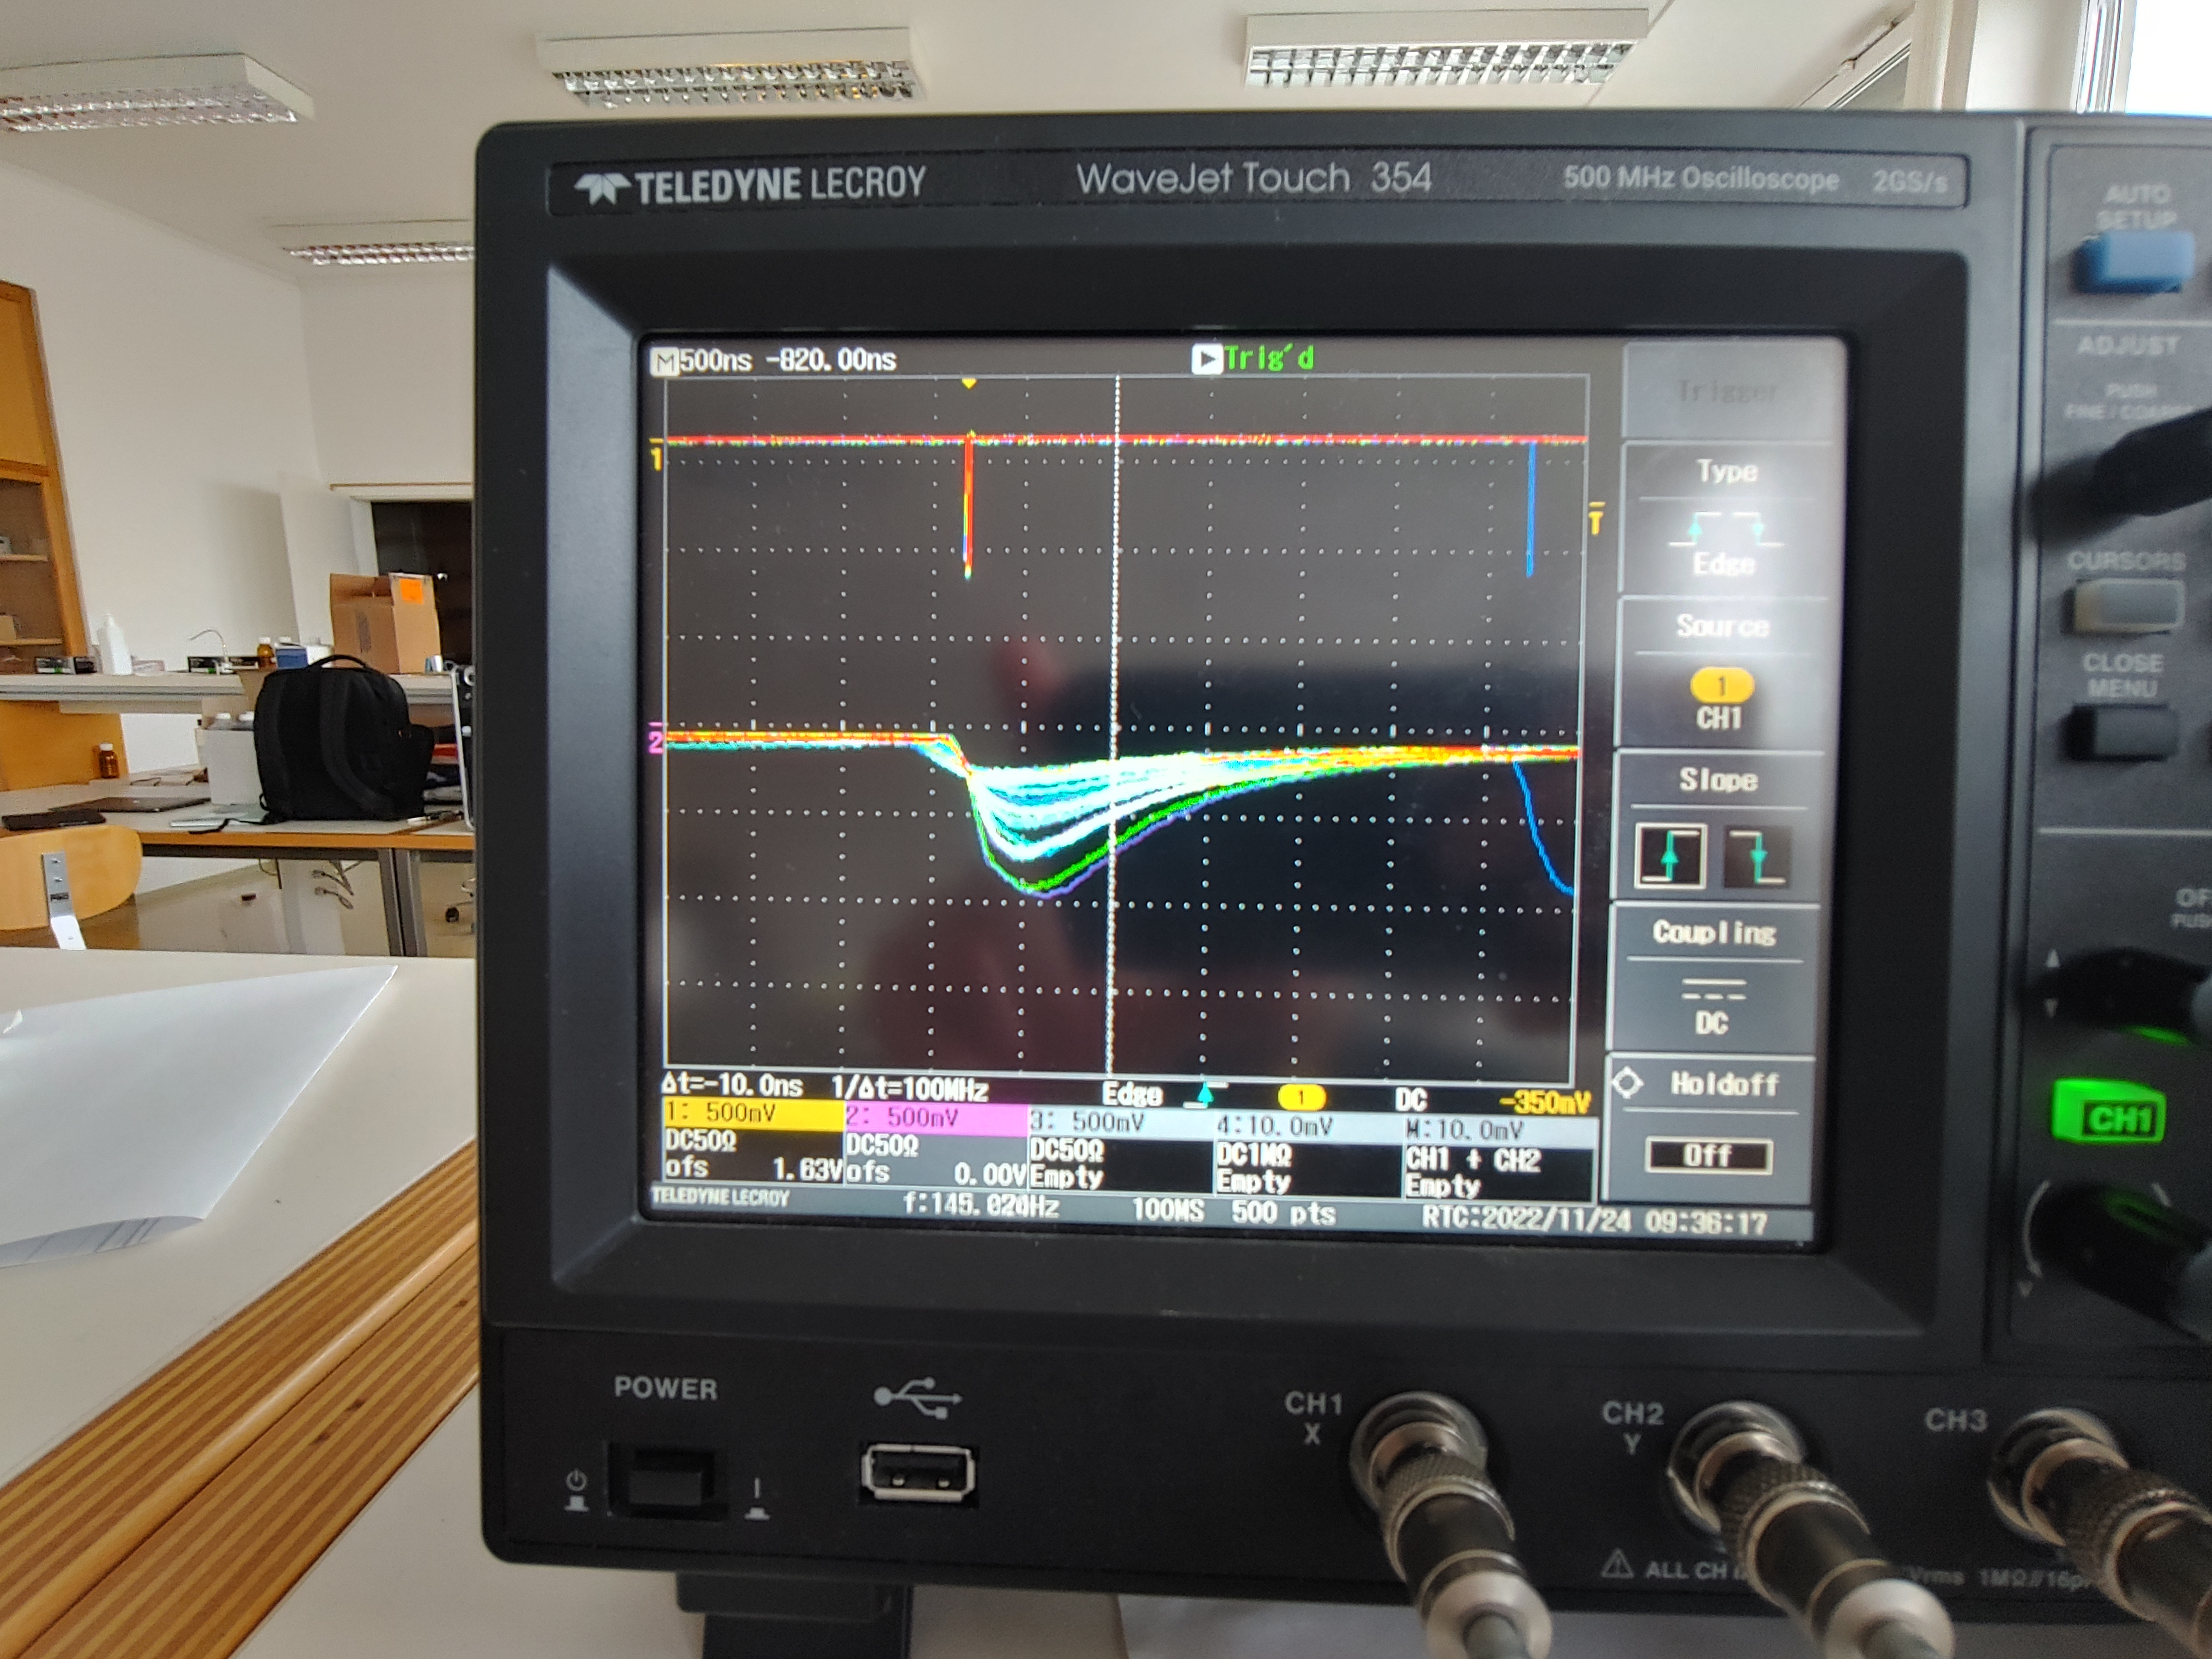
\includegraphics[width=0.5\textwidth]{signal.jpg}
    \end{center}
    \caption{Signali, sunki iz scintilacijskega detektorja na osciloscopu. Amplituda sunka je sorazmerna z energijo elektrona. Jasno vidimo, da je ena izmed energij mnogo bolj zastopana kot ostale. V nadaljnjih meritvah to pogostost kvantficiramo kot spekter.}
    \label{fig:signal}
\end{figure}

\begin{figure}
    \begin{center}
    \includegraphics{na22-lost-spectrum.pdf}
    \end{center}
    \caption{Spekter zaznanih elektronov za $^{22}\mathrm{Na}$, izražen kot gostota aktivnosti.}
    \label{fig:na22}
\end{figure}

\begin{figure}
    \begin{center}
    \includegraphics{co60-lost-spectrum.pdf}
    \includegraphics{cs137-lost-spectrum.pdf}
    \end{center}
    \caption{Spekter zaznanih elektronov za $^{60}\mathrm{Co}$ in $^{137}\mathrm{Cs}$, izražen kot gostota aktivnosti.}
    \label{fig:spectra}
\end{figure}

Spekter nato pomerimo še z večkanalnim analizatorjem, ki sledi vsem energijskim (napetostnim) intervalom hkrati (slike~\ref{fig:na22},~\ref{fig:spectra}). Pomerimo tudi spekter ozadja, ki ga kasneje odštejemo od izmerjenih spektrov. Za lažje primerjanje gledamo gostoto aktivnosti, izračunamo jo tako, da število sunkov delimo s časom (\textit{livetime}) in z dolžino energijskega intervala. Na posamezne fotovrhove prilagodimo Gaussovke oblike

\begin{equation*}
    f(x) = \frac{A_0}{\sigma\sqrt{2\pi}} e^{-\frac{1}{2} \frac{x - \mu}{\sigma^2}},
\end{equation*}

katerega površina predstavlja zaznano aktivnost tega fotovrha. Vse tako izračunane aktivnosti so predstavljene na slikah~\ref{fig:na22},~\ref{fig:spectra}. Za vzorec $^{137}\mathrm{Cs}$ poznamo začetno aktivnost $9250\,\mathrm{Bq}$, izmerjeno $9 \pm 0.25$ mesecev nazaj. Če primerjamo polovico\footnote{Pokrijemo prostorski kot $2\pi$.} te aktivnosti s površino fotovrha v~\ref{fig:spectra}, izračunamo, da je učinkovitost našega detektorja

\begin{equation*}
\eta = (5.2 \pm 0.1)\,\%.
\end{equation*}

Za vse energije gamma fotonov izračunamo še predvidene položaje Comptonskega \textit{backscattering} vrha in jih prikažemo na~\ref{fig:na22},~\ref{fig:spectra}.

\end{document}
